\section{Linear Algebra}

\begin{definition}[Basis]
    Given a set of vectors in $\mathbf{R}^{n}, V$, which is linearly
    independent, the set $V$ is a \textit{basis} if you can span 
    $\mathbf{R}^{n}$ using $V$.
\end{definition}

\begin{definition}[Backward substituion]\label{backwardsubstituion}
    Opposite of~\nameref{forwardsubstituion}.
\end{definition}

\begin{definition}[Condition number]\label{conditionnumber}
    A measure of how the output value for a function changes respective to 
    input variables.
\end{definition}

\begin{definition}[Column space]
    All linear combinations of the columns of a matrix $A$.
\end{definition}

\begin{definition}[Consistent]
    $\iff$ the rightmost column of an augmented matrix is not a pivot column.
    I.e.\ in a 3x4 matrix, if the last row is zero and 2nd column has pivot
    column, then the system is still consistent.
\end{definition}

\begin{definition}[Diagonal Dominance]
    $\forall{i}, \exists{i} A_{i, i}, \forall i, \iff A_{i,i} 
    \geq \sum\limits_{j = 0, j\neq i}^{m}$,
    then matrix $A$ is DD.
\end{definition}

\begin{definition}[Diagonlizable matrix]
    Given a matrix $A$, we can express it as $A = PDP^{-1}$.
    Then, we can compute:
    \begin{align}
        A^{2} = (PDP^{-1})(PDP^{-1}) = PD(P^{-1}P)DP^{-1} = PDDP^{-1} \\
        \text{Because} P \cdot P{-1} = I \\
        \dots A^{k} = PD^{k}P^{-1}
    \end{align}

    So, we use diagonal matrices to easily raise matrices to power $k$.
    
    To diagonalize a matrix $A^{n\times{n}}$, it is required that it has $n$ linearly 
    independent eigenvectors.
\end{definition}

\begin{definition}[Divergence]
    In vector calculus, divergence measures the magnitude to the
    gradient of~\nameref{vectorfield}s at a given point.

\end{definition}

\begin{definition}[Dotting matrices]
    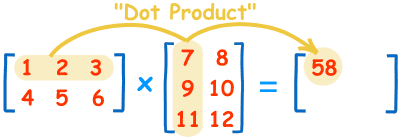
\includegraphics[scale=0.3]{mm.png}
\end{definition}

\begin{definition}[Echelon form]
    A matrix where:
    \begin{enumerate}
        \item All nonzero rows are above zero-rows
        \item Each pivot column is placed from left to right
    \end{enumerate}
\end{definition}

\begin{definition}[Eigenvector]\label{eigen}
    Given a square matrix A, when A is multiplied with an eigenvector $v$,
    the resulting matrix A${^\prime}$ is a multiple of $v$.
    The multipe is denoted by $\lambda$ and is called an eigenvalue.
    So, $Av = \lambda v$

\end{definition}

\begin{definition}[Forward substituion]\label{forwardsubstituion}
    In an iterative method, if we first solve an element $A_{i,j}$,
    then when we caluclate some $A_{i+a, j+b}$ in the same iteration, then we
    use the updated value of $A_{i,j}$. Opposite
    of~\nameref{backwardsubstituion}

\end{definition}

\begin{definition}[Gaussian Elimination]
    AKA ``Row reduction''. Add row $x$ to row $y, y \neq x$, to reduce $y$ to 
    zeroes.

\end{definition}

\begin{definition}[Ill-conditioned matrix]
    A matrix is ill-conditioned if the~\nameref{conditionnumber} is large.
    If you make a small change in an ill conditioned matrix, there are usually
    large differences in results from calculations with this maxtrix.

\end{definition}

\begin{definition}[Inner product]\label{innerprod}
    The product $u^{T}v$. Given that $u, v \in R^{i\times{j}}$, then we need to transpose
    to perform normal dot products.

    Inner products are commutative: $u \dot v \equiv v \dot u$.
\end{definition}

\begin{definition}[Inverse]
    For a matrix $A \in \mathbf{R}^{2x2}$:
    $$
    A^{-1} = \frac{1}{|A|}
    \begin{bmatrix}
    d & -b \\
    -c & a
    \end{bmatrix}
    = \frac{1}{ad - bc}
    \begin{bmatrix}
    d & -b \\
    -c & a
    \end{bmatrix}
    $$
    For a matrix $A \in \mathbf{R}^{3x3}$: bcacab

    Properties:
    \begin{itemize}
    \item $(A^{-1})^{-1} = A$
    \end{itemize}
\end{definition}

\begin{definition}[Kernel]
    For a vector space given by a~\nameref{lintrans}, a kernel is the set
    of vectors $v \in V$, s.t. $T(u) = 0$.
\end{definition}

\begin{definition}[Length of Vector]\label{vectorlength}
    For a vector 
    \begin{align*}
        v = [a_{1}, a_{2}, \dots , a_{n}] \\
        |v| = \sqrt{a^{2}_{1} + a^{2}_{2} + \dots + a^{2}_{n}}{}
    \end{align*}
\end{definition}

\begin{definition}[Linear dependence]
    For $V = {v_{1}, \dots, v_{n}}$, and $\forall v, v is vector$,
    if none of the vectors in V can be written as a linear combination
    from the other vectors in V, the set is linearly independent.
\end{definition}

\begin{definition}[Linear transformation]\label{lintrans}
    Take a vector space into another, s.t.\
    \begin{align}
        T(u + v) = T(u) + T(v) &\forall u,v \in v \\
        T(cu) = cT(u) &\forall u \in V
    \end{align}
\end{definition}

\begin{definition}[Matrix of observations]
    Collect a sample, subject it to tests, and for each test, you give a value.
    For $n$ tests and $m$ samples, you will result in $\Re^{n\times{m}}$ 
    \textit{matrix of observations}.
\end{definition}

\begin{definition}[Norm]
    The ``length'' of a vector, just remember to sum up over all dimensions.
    Each number is raised to $n$, and the total sum is then raised to

    \begin{description}
        \item[L1]
        \item[L2] Can be defined as:
            \begin{align}
                \phi^{2} = \phi \times \phi =
                \dots = \int{\phi (x)^{2}  dx} \\
                |x| = \sqrt{ \sum\limits_{k = 1}^{n}{x_{k}|^{2}}}
            \end{align}
    \end{description}

    $\frac{1}{p}$.  
\end{definition}

\begin{definition}[Normalization of vectors]
    $ \hat{X} \equiv \frac{X}{|X|} $, where $|x|$ is the~\nameref{vectorlength}
    $X$ is, in this case, evaluated as the additive sum of it's entries.
\end{definition}

\begin{definition}[Null space]
    Given a matrix $A$, if you solve for that each row = 0,
    all possible values for each $x$ makes out the Null space.

    Note that here it is apossible to get free variables for 
    some x, and bound to others.

\end{definition}

\begin{definition}[Numerical stability]
    This concept describes how changes in the input should not affect the result.
    An example could be that sorting a list should not change the outcome from
    applying a function to the input.
\end{definition}



\begin{definition}[Orthogonal]\label{orthogonal}
    Two lines that intersect each other at 90 degrees.\\
    \begin{itemize}
        \item Orthogonal matrices preserve dot products:
        given two vectors $u$, and $v$, and an orthogonal matrix Q,
        the following is true:
        $u \times v = Qu \times Qv$
        \item The determinant of an orthogonal matrix is always 1 or -1
        \item The transpose of $Q$ is equal to it's inverse, hence:
            $Q \times Q^{T} = I$
    \end{itemize}
\end{definition}

\begin{definition}[Orthonormal]
    In~\nameref{innerprod} space are orthonormal if they are
    orthogonal and unit vectors.
\end{definition}


\begin{definition}[Perpendicular]
    Similar to~\nameref{orthogonal}, but with lines.
\end{definition}

\begin{definition}[Pivoting]
    Finding the first non-zero element in an algorithm on linear systems.
    To do so, you can do things like gaussian elimination, etc.
    \begin{description}
        \item[Complete pivoting] find the largest absolute value of a pivot,
            considering all elements.
        \item[Partial pivoting] finds the largest absolute value in the pivot
            column.
        \item[Scaled pivoting] finds the largest absolute value of a pivot
            column relative to it's entries in the same row.
    \end{description}
\end{definition}

\begin{definition}[Plane]
    A flat, two-dimensional surface
\end{definition}

\begin{definition}[Positive semidefninite matrix]
    Properties:
    \begin{itemize}
        \item Nonnegative~\nameref{eigen}s
        \item $X = V^{T}V$ for some $V \in \mathbf{R}^{mxn}$
        \item $X = \sum\limits_{i=1}^{m}\lambda_{i}w_{i}w^{t}_{i}$ 
            for some $\lambda_{i} \geq 0$ and vectors $w_{i} \in \mathbf{R}^{n}$
            such that $w^{T}_{i}w = 1$ and $w^{T}_{i}w_{j} = 0$

    \end{itemize}
\end{definition}

\begin{definition}[Preconditoner]
    A matrix $P$ such that $P^{-1}A$ has a smaller~\nameref{conditionnumber}
    than $A$.

\end{definition}

\begin{definition}[Projection]
    define a vector $v$ and $u$.
    \begin{align*}
        L &= \left\{cv | c \in \mathbf{R} \right\}  \\
        proj(v) &= l \in L \text{\ such that\ } u - proj(v) 
        \text{\ is~\nameref{orthogonal} to l}  \\
        \textit{I.e., } proj(v) &= cv, c \in \mathbf{R}
    \end{align*}

    Properties:
    \begin{itemize}
        \item $proj(v) = proj(v)^{2}$
        \item Linear independence on $u, v$ also relates for $v - proj(v), u$
        \item adding $proj(v)$ to $v$ gives you $u$
    \end{itemize}

\end{definition}

\begin{definition}[Relaxation methods]
     relaxation methods are iterative methods for solving systems of equations,
     including nonlinear systems. Examples are Gauss-Seidel, Jacboi, etc.

\end{definition}

\begin{definition}[Singular matrix]
    Any square matrix without an inverse.
    A matrix is singular $\iff$ its determinant is 0.

\end{definition}

\begin{definition}[Span of vectors]\label{vectorspan}
    All linear combinations of a set of vectors.
    \begin{align*}
        V &= \left\{v_{1}, \dots, v_n\right\} \\
        C &= \left\{c \in C | \mathbf{R}\right\} \\
        span &= c_{1}v_{1} + \dots + c_{n}v_{n}
    \end{align*}
\end{definition}

\begin{definition}[Spectrum of a matrix]
    The multiset of its eigenvalues
\end{definition}

\begin{definition}[Spectral Radius]
    The largest absolute eigenvalue of a matrix.
\end{definition}

\begin{definition}[Successive Over Relaxation]
    Gauss-Seidel is the same as SOR (successive over-relaxation) with $\omega=1$
\end{definition}

\begin{definition}[Symmetric]
    \begin{itemize}
        \item Length of rows is equal
        \item The transpose is equal to the originl
    \end{itemize}
\end{definition}

\begin{definition}[Tensor]
    Geometric objects that describe linear relations between vectors or scalars.
\end{definition}

\begin{definition}[Toeplitz matrix]
    $$
    \begin{bmatrix}
    a & b & c & d \\
    b & a & b & c \\
    c & b & a & b \\
    d & c & b & a
    \end{bmatrix}
    $$

    Noteworthingly, this kind of matrix can be inverted in $O(n \times \log{n})$
\end{definition}

\begin{definition}[Trace]
    Sum of all diagonal entries in a matrix.
    $A_{11} + A_{22} + A_{nn}$
\end{definition}

\begin{definition}[Transpose]
    Take column $i$ and make it into a column. Repeat.
\end{definition}

\begin{definition}[Unit vector]
    A vector who's length is 1.
\end{definition}


\begin{definition}[vector length]
    number of "steps" in a vector
\end{definition}

